\documentclass{ML}
\usepackage{amssymb}
\usepackage{latexsym}
% 姓名,学号
\infoauthor{朱明彦}{1160300314}

% 课程类型,实验名称
\infoexp{课程类型}{概述}

\infoschool{计算机学院}{高宏}

\begin{document}
\maketitle

\tableofcontents
\newpage

\begin{center}
    \textbf{\zihao{3} 论文概述}
\end{center}

\section{解决的问题}
选择的论文\cite{toain}为2018年PVLDB上面的一篇文章,\textbf{主要解决的问题是Road Networks上面动态的kNN查询}。

针对这个问题,作者主要有如下\textbf{三个方面}的工作:
\begin{enumerate}
    \item 对于Road Networks上需要进行kNN查询的系统建立新的数学模型,并找到其中影响系统整体吞吐量的关键因素。
    \item 建立了一个以Shortcut Graph为基础的索引,SCOB。
    \item 设计了可以根据Update/Query的所用时间动态调整SCOB以最大化系统吞吐量的算法,TOAIN。
\end{enumerate}
\section{采用的思想}
作者为了解决Road Networks上面动态的kNN查询,采用的思想是\textbf{先明确系统的目标(最大化系统的吞吐量),建立数学模型衡量寻找影响体统吞吐量的关键因素,对于关键的因素建立索引并利用设计的算法尽量提高关键因素影响下的部分,最终实现最大化吞吐量的目的}。

\begin{figure}[htb]
	\centering
	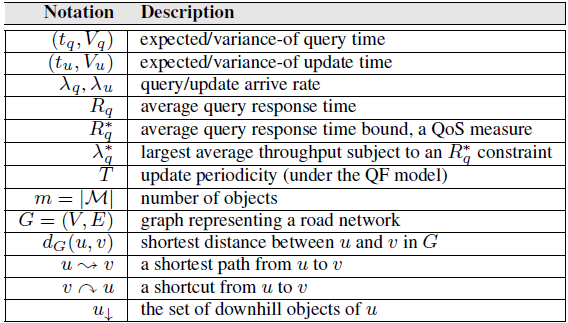
\includegraphics[width=0.8\linewidth]{media/notations.png}
	\caption{Notations}\label{fig:notations}
\end{figure}
\subsection{数学模型方面}
作者主要考虑了两种不同的情况,分别对应于现实中两种不同的应用,即\textbf{如滴滴类似的打车软件系统和捕捉精灵球的Pokemon}。 作者在考虑数学模型时,从\textbf{Query}和\textbf{Update}分别考虑其影响,然后针对这两种不同的应用区分它们在Query和Update上面的差别,从而建立起来不同的数学模型。

\textbf{以下两种应用都假设所有的查询到来是随机的,论文中为了方便假设Query符合泊松过程(Poisson Process)。}
\subsubsection{打车软件(BUA+QF Model)}\label{sec:bua_qf}
\textbf{BUA(Batch Update Arrival)模型是针对Update操作来说},其假设所有的元素都会进行Update操作,且都是在时间片的开始时刻进行,如果在某一个时间片里没有完成相应的Update操作,则直接舍弃未做操作,进行下一轮操作即可。\textbf{QF(Query First)是针对系统中队列模型来说的},其假设Query在队列中的优先级高于Update。

基于上面的假设,在打车软件这样的系统中,对于每个Query是来自用户的,查询在其附近最近的K个车辆;每个Update是来自汽车的,其在指定间隔内向系统返回其最新的位置。这样,高优先级的Query可以尽量减少用户请求的查询的延迟,并且丢失少量Update使得某些车辆的信息具有很短距离的差距,所以这样的假设对于该应用是合理的。

利用在\cite{single-server-queue}中的结论,可以得到式\eqref{equ:1},其中$R_q$为平均查询响应时间,$t_q, V_{q}$分别是查询时间的期望和方差,$\lambda_{q}$为Query到达的速率,即泊松过程中的参数。
\begin{equation}
R_{q}=\frac{\lambda_{q}\left(t_{q}^{2}+V_{q}\right)}{2\left(1-\lambda_{q^{t} q}\right)}+t_{q}
\label{equ:1}
\end{equation}

通过式\eqref{equ:1}可以看到,\textbf{整体的查询响应时间随$\lambda_{q}$的增大而增大,这也与我们的直觉相符合,说明此模型具有一定的道理}。进而通过两个约束,\textbf{查询的响应时间不能超过用户能够忍受的最大值}和\textbf{在一个时间间隔内需要最少的用于Update的时间限制},得到最终的$\lambda_{q}$的上界,如式\eqref{eq:2}所示。

\begin{equation}
\lambda_{q}^{*} \leq \min \left\{\frac{2\left(R_{q}^{*}-t_{q}\right)}{V_{q}+2 R_{q}^{*} t_{q}-t_{q}^{2}}, \quad\left(T-m t_{u}\right) /\left(T \cdot t_{q}\right)\right\}
\label{eq:2}
\end{equation}

为了可解释性,将式\eqref{eq:2}转化为式\eqref{eq:3}。
\begin{equation}
\lambda_{q}^{*} \leq \left\{
\begin{array}{lll}
{1 / t_{q},} & {\text { if } \alpha \beta<1 / 2} & {(\text { QoS-bound mode })} \\ 
{(1-\beta) / t_{q},} & {\text { if } \alpha \beta \geq 1 / 2} &\text {(Update-bound mode)}
\end{array}
\right.
\label{eq:3}
\end{equation}

其中$\alpha=R_{q}^{*} / t_{q} ; \quad \beta=m t_{u} / T ; \quad \gamma=V_{q} / t_{q}^{2}$;$\alpha$用来衡量平均查询相应时间的上界与平均查询时间的比值,$\beta$用来衡量一个时间片内处理Update所用时间的占比,$\gamma$是离散系数(coefficient of variation)的平方,相对于标准差其为无量纲量可以用在不同的索引算法中进行比较,一般$\gamma \in [0.1, 0.9]$。	

\subsubsection{Pokemon游戏(RUA+FCFS模型)}
对于pokemon类似的以所在位置为中心,查询周围存在的Pokemon,并进行捕捉的这类游戏,其Update不是按照某一指定的时间间隔返回的,而是随机的,所以其Update操作不能在使用BUA模型,而是转为RUA(Random Update Arrival)模型,同样的为了方便研究,\textbf{作者假设RUA的Update符合另一个泊松过程(与Query到来的泊松过程不同)}。

对于Query的优先级,Pokemon游戏很注重每个Pokemon的位置更新,所以该模型的队列模型使用了FCFS(First-come-first-served),即Query和Update具有相同的优先级,根据到来的顺序来进行操作。

其分析过程与\ref{sec:bua_qf}节类似,最终得到式\eqref{eq:rua_fcfs},衡量在该模型下的Query到来频率的上界。

\begin{equation}
\lambda_{q}^{*} \leq \min \left\{\frac{2\left(R_{q}^{*}-t_{q}\right)\left(1-\lambda_{u} t_{u}\right)-\lambda_{u}\left(V_{u}+t_{u}^{2}\right)}{V_{q}+2 R_{q}^{*} t_{q}-t_{q}^{2}}, \frac{1-\lambda_{\mathrm{u}} t_{u}}{t_{q}}\right\}
\label{eq:rua_fcfs}
\end{equation}

\subsection{索引SCOB方面}
在索引和算法方面,作者做出了两个假设,这两个假设虽然在后面进行了放松,但本质上论文作者最终解决的问题也没有彻底摆脱这第一个假设的约束,这一部分在后面%TODO 
详细来说。两个假设分别是:
\begin{enumerate}
	\item 抽象后的图G是无向图
	\item 所有节点的Rank是不一样的
\end{enumerate}

\subsubsection{符号定义}
\paragraph{SHORTCUT SET $SC_{<}$} 给定一个图$G=(V, E)$和一个定义在$V \to \mathbb{N}$上的Rank Function,则一条捷径(shortcut)$u \curvearrowright v \in SC_{<}$当且仅当1.$u, v \in V$,2.$r(u) < r(v)$,3.对于从$u$到$v$上最短路上的中间任意节点$z$均有$r(z) < r(u)$。

从上面的定义我们可以直接得到一个结论,如式\eqref{lemma:3},其中$SC_{<}$是从$G$上导出的捷径图(shortcut graph),因为不一定所有的$G$上的最短路都符合$r(z) < r(u)$即上述定义的第3条规则。
\begin{equation}
d_{G}(u, v) \leq d_{SC_{<}}(u, v) \quad \forall u, v \in V
\label{lemma:3}
\end{equation}
\paragraph{SUMMIT NODE}
给定一个最短路径(shortest path)$s \leadsto t$,则对于该最短路的Summit Node是$s \leadsto t$上具有最高权重的节点。

根据$SC_{<}$和summit node的定义以及第一个假设,我们可以直接得到式\eqref{lemma:4},其中$x$是最短路径$s \leadsto t$上的summit node。
\begin{equation}
d_{G}(s, t)=d_{SC_{<}}(s, x)+d_{SC_{<}}(t, x)
\label{lemma:4}
\end{equation}
\paragraph{DOWNHILL OBJECTS}
论文中作者为了形象表示不同节点的rank不同,具有越高rank的节点在图中的位置越高,如图\ref{fig:downhill}所示。基于这种形象的表示,如果在$SC_{<}$中有一条从$v$指向$u$的shortcut,则称$v$是$u$的downhill object。
\begin{figure}[htb]
	\centering
	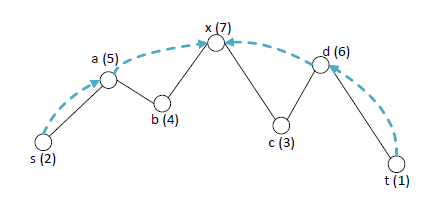
\includegraphics[width=0.6\linewidth]{media/downhill.png}
	\caption{Query Algorithm}\label{fig:downhill}
\end{figure}
\paragraph{$\mathbf{kDNNs}$}
给定一个节点$u \in G$,离它最近的k个downhill objects被记作$kDNN(u)$。

\subsubsection{基本思想}
根据式\eqref{lemma:3}和$G$是无向图的假设,可以有结论\textit{给定一个节点$s$和一个位于节点$t$的物体$o$,如果$o$是$s$的kNN之一,则有$o \in kDNN(x)$,$x$是最短路$s \leadsto t$上的summit node}(其证明使用了证明其逆否命题的方法,主要利用三角不等式、式\eqref{lemma:3}进行放缩)。\textbf{通过以上结论,可以利用kDNN和一些特定的summit node可以得到一些源点的KNN结果。}

SCOB索引本质上也是利用了Dijkstra在图上进行搜索,而传统的方式对于一个有M个节点的图,需要进行M次s-climb(从源点到summit node的搜索)以及M次t-climb(从目标点到summit node的搜索);而使用了SCOB索引\textbf{在每个summit node上记录在Shortcut Graph中的k个最近的downhill objects的id和其距离,以减少s-climb(t-climb)的次数,来提高效率,最终实现了仅需要从Query发出的节点进行一次s-climb就可以找到对应这次Query的kNN结果}。

具体如何维护SCOB索引,见\ref{sec:scob_index}节。
\subsection{算法TOAIN方面}
\section{基本算法描述}
文中以伪代码形式讲述的算法共有4个,下面将分别进行描述。
\subsection{SCOB Index}\label{sec:scob_index}
\paragraph{Query}
\begin{figure}[htb]
	\centering
	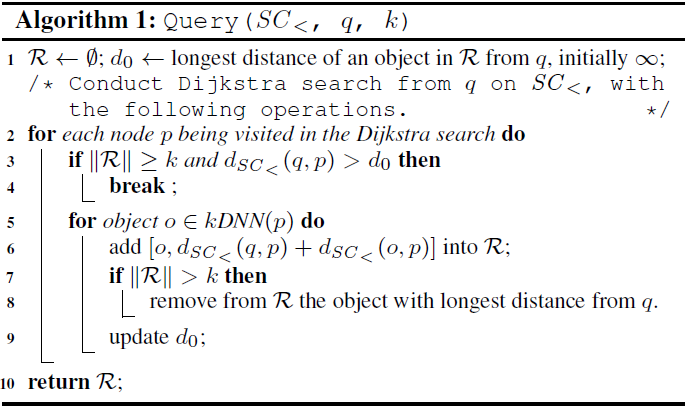
\includegraphics[width=0.8\linewidth]{media/query.png}
	\caption{Query Algorithm}\label{fig:query}
\end{figure}
\paragraph{Insert}
\begin{figure}[htb]
	\centering
	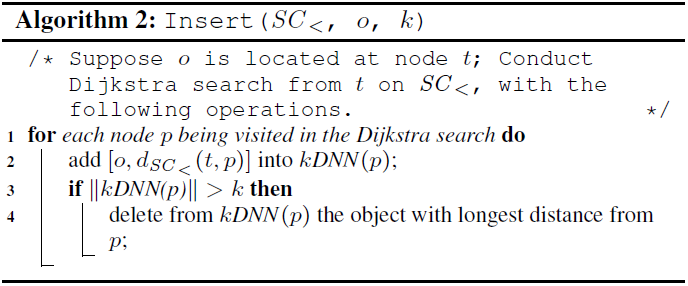
\includegraphics[width=0.8\linewidth]{media/insert.png}
	\caption{Insert Algorithm}\label{fig:insert}
\end{figure}
\paragraph{Delete}
\begin{figure}[htb]
	\centering
	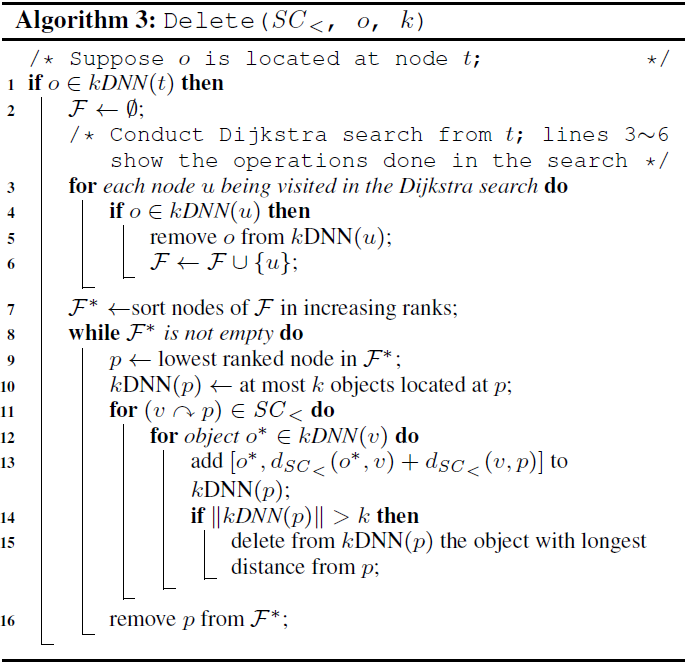
\includegraphics[width=0.8\linewidth]{media/delete.png}
	\caption{Delete Algorithm}\label{fig:delete}
\end{figure}
\subsection{TOAIN}
\paragraph{Compute Rank}
\begin{figure}[htb]
	\centering
	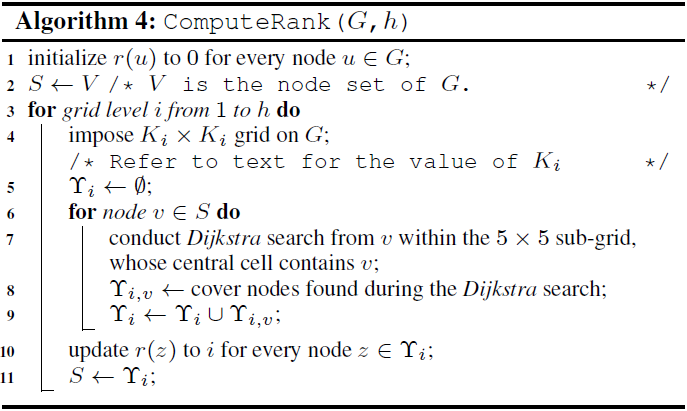
\includegraphics[width=0.8\linewidth]{media/compute_rank.png}
	\caption{Compute Rank Algorithm}\label{fig:compute_rank}
\end{figure}
\section{算法分析}

\section{举例说明}

\appendix

% \section{源代码}
% \section{参考文献}
\begin{thebibliography}{20}
    \bibitem{toain} Luo, S., Kao, B., Li, G., Hu, J., Cheng, R., \& Zheng, Y. (2018). TOAIN: a throughput optimizing adaptive index for answering dynamic k NN queries on road networks. Proceedings of the VLDB Endowment, 11(5), 594-606.
    \bibitem{single-server-queue} J. W. Cohen. The single server queue, volume 8. Elsevier, 2012.
\end{thebibliography}

\end{document}
